\section{System Overview}

For ease of adoption, we have designed Shark to be entirely hot-swappable with Hive. Users can run Shark in an existing Hive warehouse. Queries will return the same set of results in Shark, albeit much faster in most cases, without any modification to the data or queries themselves.

We have implemented Shark using Spark, a system that provides the RDD abstraction through a language-integrated API in Scala, a statically typed functional programming language for the Java VM. Each RDD dataset is represented as a Scala object, while the transformations are invoked using methods on those objects. 

A Shark cluster consists of masters and workers. A master's lifetime can span one or several queries. The workers are long-lived processes that can store dataset partitions and intermediate RDDs resulting from transformations in memory across operations. When the user runs a query, the client connects to a master, which defines RDDs for the workers and invoke operations on them. %[Mention Mesos here?]

Figure \ref{fig:arch} shows the general architecture of Shark. Data is stored physically in the underlying distributed file system HDFS. Shark uses the Hive metastore without modification to track table metadata and statistics, much like the system catalog found in traditional RDBMS. The Shark CLI driver replaces the Hive CLI and invokes the Shark runtime driver. The Shark runtime uses Hive's functionality for parsing and compilation of HiveQL queries into a query plan. This query plan is then passed to Shark operators, which use Spark, which is loaded as a library, to create and transform RDD representations of the table data. Caching is done at the operator level by serializing query plan operator subtrees and enabling persistence on RDDs.

\begin{figure}[t]
	\centering
	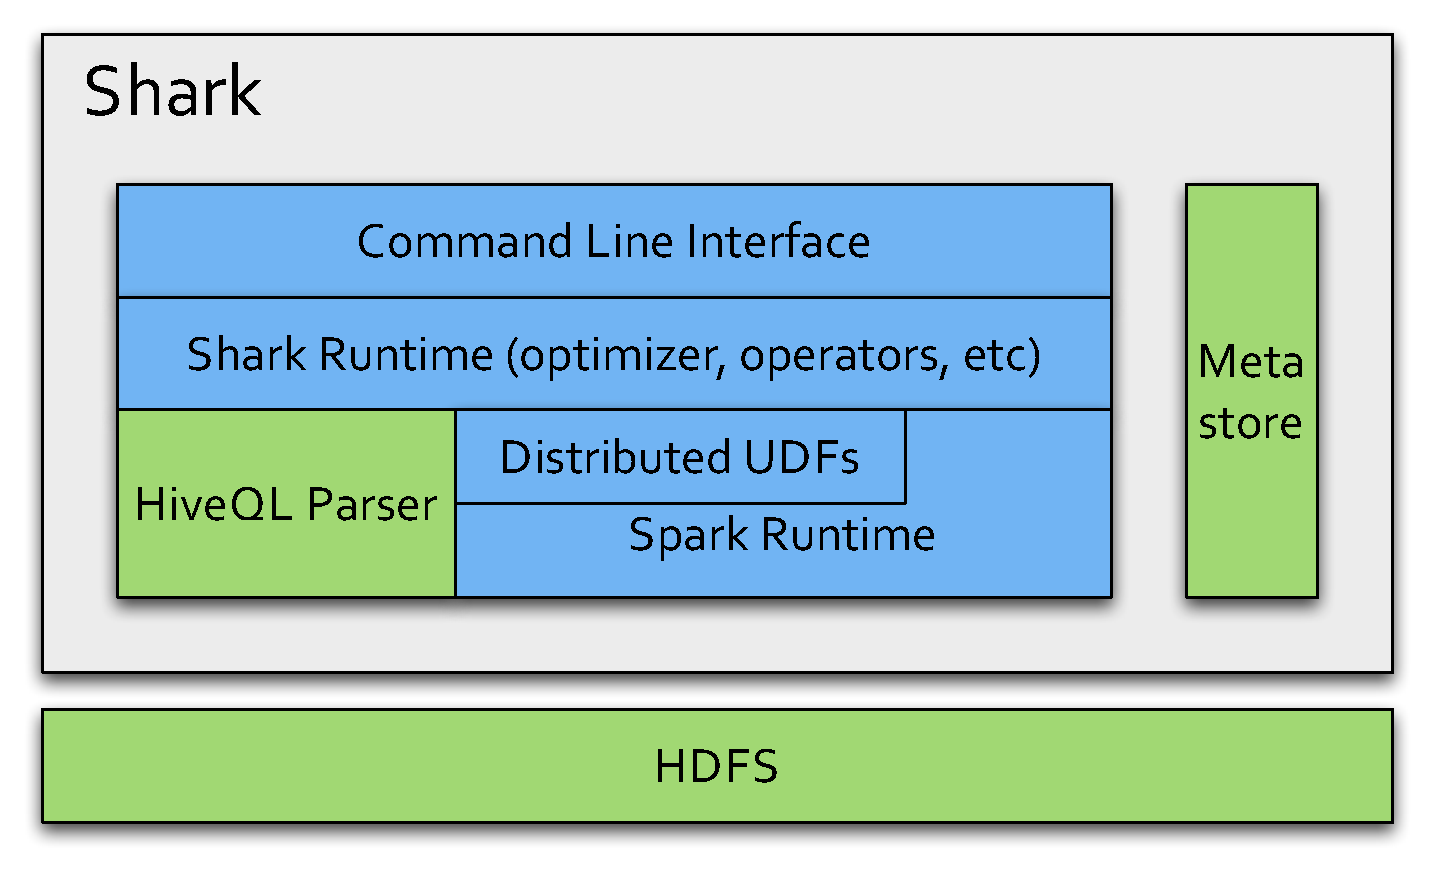
\includegraphics[width=\linewidth]{files/architecture.pdf}
	\caption{Shark Architecture}
	\label{fig:arch}
\end{figure}
